\documentclass[a4paper,11pt]{article}
\title{COSC345 Project Proposal}
\author{Richie, Shaun, Chris, Tom, Reuben}
\date{\today}
\addtolength{\oddsidemargin}{-.5in}
\addtolength{\evensidemargin}{-.5in}
\addtolength{\textwidth}{1in}

\addtolength{\topmargin}{-.875in}
\addtolength{\textheight}{1.75in}

%\includegraphics
\usepackage{graphicx}
\usepackage{multicol}
\usepackage{listings}
\lstset{language=Python} 

\begin{document}
\maketitle

%THE FAMOUS FIVE
%\\*Project Proposal
%\\*Prepared for: Andrew Trotman, Lecturer
%\\*Prepared by: The Famous Five
%\\*26 March 2014
%\\*Proposal Name: Five Make a Unicorn Shell
%\\*THE FAMOUS FIVE
\section{Overview}

The Unicorn Shell (working title) will be a modern, POSIX style shell which will be released on linux, OSX and Windows under the FreeBSD License. The project will written almost entirely in C++ and al the source code will be released in it's entirety.

The Unicorn Shell will be targeted at those of beginner level, people who are not particularly skilled at using a shell, and possibly even those who have never used one before.

The shell will be developed to be intuitive. Basic shell operations will be natural interactions, that most computer users are familiar with, anyone will be able to pickup unicorn very quickly, even those from different OS backgrounds.

Despite the target audience of our Shell, it will still provide the full feature set that advanced users would expect.

Such features will include tab-completion, inline command prediction and detection, stream redirection, fine grained multi process control, several predefined macros and aliases for things like accessing the command history. And almost everything will be able to be customised.

It will also look pretty with proportional width font, no more ugly monospaced grabage, only the most beautfilly kerned Helvetica. 

\section{Introducion}
Thank you for choosing to read our project proposal

We are INSERT NAME HERE and we are extremely excited to show you our proposal. When set with the task of designing and creating a new shell we had a number of ideas that sprang to mind and a great deal more that became more apparent to us as we researched shells in greater detail and found things that we felt a shell would benefit from having.
\pagebreak
\section{Team Summary}

\subsection*{Reuben Crimp (Surgeon):}
Reuben began programming in high school, making what interested him, games and websites. He graduated highschool doing well in mathematics. He enrolled at Otago University in mid 2012, majoring in computer science, with a minor in mathematics. He has very little industry experience but a strong passion for the subject matter.

\subsection*{Shaun Wratten (Co-pilot):}
Shaun recently graduated from UCOL in Palmerston North with a Bachelor’s degree in Information and Communications Technology, in which he learnt a decent portion of his skill set. This includes programming in C\#, C++, scripting and web design using PHP and Javascript, and working with MS-SQL and MySQL database. One of the major things he learnt while studying was how to strutter a team project and hot to be as successful leader and team member.

\subsection*{Chris McMillan (Toolsmith):}
Chris has studied at the University of Otago since 2010, but only became interest in computers after high school. He completed a chemistry degree and then decided that his passion lay in computers and began study towards a computer science major as well. He will finish his BSc double major at the end of 2014. His main strengths are music and audiosoftware. Chris can confidently write Java and Python programs, but building a shell in C++ will be a challenge for him that he looks forward to and hopes to learn a lot from.

\subsection*{Thomas Hall (Lanuage Guru and Tester):}
Thomas is a recent graduate with BSc in Physics. He is currently studying a DipGrad in computer science to be finished in early 2015. He has experience programming in C\# from experimenting with Unity, and Matlab as part of his physics education. He also has a experience with Java and Python.

\subsection*{Richie McKee (Editor and Program Clerk):}
Richie completed his LLB/BA at the end of 2012 at Otago University. He always had a strong desire to learn computer science but is only now taking steps towards doing so. He began his DipGrad at the start of 2014 and hopes to be completed by the end of the year. As such his current level of experience is limited and his experience with programming is limited to what he learnt during Summer School and what he is currently covering throughout the semester. To him the project is a daunting but exciting prospect that he hopes to learn from.
\pagebreak
\section{Project Description}

We want a shell that has all the features of popular shells like the Bourne Again Shell. However we will attempt to add features that make it far more usable and also include additional features that make our shell standout, encouraging people to adopt our obviously superior piece of software.

\section{Tools and Hardware}

\subsection*{Windows:}
IDE/compiler: Visual Studio 2013 Professional
lang: standard c++ libraries and standard windows libraries included with VS’13.
GUI: WIN32

\subsection*{OSX:}
IDE/compiler: Xcode
lang: standard C++ libraries
GUI: Cocoa graphics, in Objective C

\subsection*{Linux:}
compiler: g++
lang: standard C++ libraries
GUI: X11

We will use git for our distributed revision control, with project hosting by the generous people at github.

\section{The Shell}

Our shell will support stream redirection and piping

Features:
Windows, Linux, OSX platforms
Pipes and redirects | < >
Support proportional spaced fonts for the CLI
Highlight text, cut, copy, paste
Mouse interaction
Syntax highlighting, (gre, grep)
support aliases (user defined command shortcuts)
resizable window
Associate *.sh files with our shell
Optional Features:

\begin{center}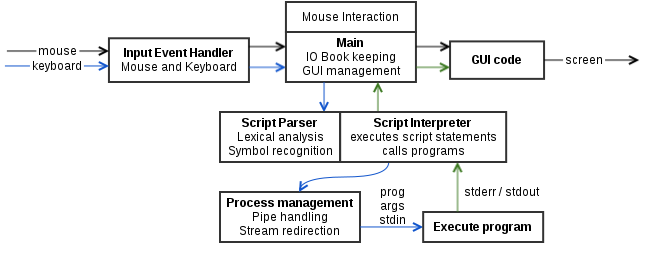
\includegraphics[width=16cm]{shellflow.png}

Fig 3: The flow of information through the shell's modules\end{center}

Different operating systems by convention define a new line within a file differently
We will allow the user to choose how to handle cross platform files
Fix:	

edit as current OS, save as current OS (Forced when parsing a script)
Compatibility: 	
edit as current OS, save as original.
Do nothing: 	 edit as original save as original.
Custom: 	
Fix; but you can specify the replacement terminator {‘\textbackslash r’, ‘\textbackslash n’, ‘\textbackslash r \textbackslash n’, ‘\textbackslash n \textbackslash r’}

Script syntax and semantics definition
like python, but with braces? i.e. fuck the strict use of whitespace.
like Bash, but more strict, like C? i.e. fuck the vague million+ ways to do things







\subsection*{Usability Features}
The shell will allow for intuitive mouse interactions, these interactions will be very similar to the actions in a standard GUI OS environment (i.e. double click for open).

However, most of our actions wont actually perform the action outright, instead it will paste the command that would perform the requested action into the current prompt, i.e. clicking "delete file" in a *nix environment will paste the command "rm \textless file-name\textgreater" into the prompt, the user will then have to press "return" to execute the command.

The purpose of this is to help the user if they do not know the specific text command, and then to teach that particular command to them.


\begin{center}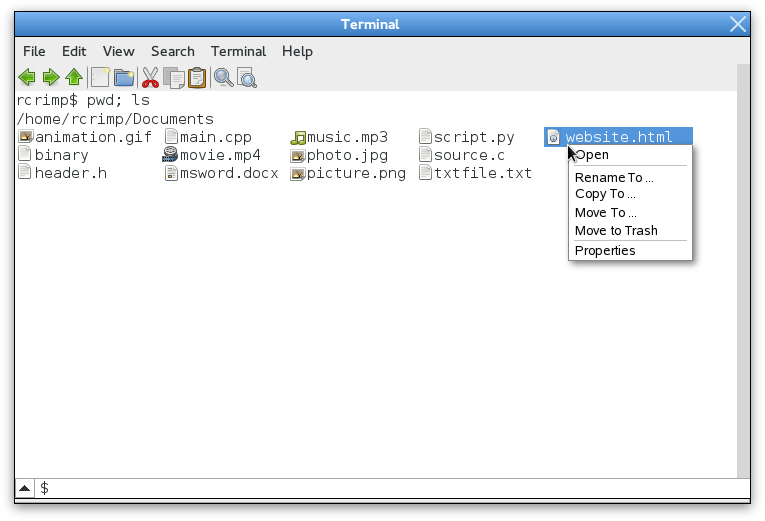
\includegraphics[width=12cm]{context.png}

Fig 1: graphical ls with context menu\end{center}

Our shell will come with an inbuilt 'ls' function, designed specifically to aid beginners
(which is replacable with the OS default ls/dir)
\\*File-names will be preceded by a filetype icon, like a GUI shell, see (fig.1)

\subsection*{Intuitive directory navigation}
Clicking on a directory will paste the command "cd \textless dir-name\textgreater" into the prompt.
\\*Double clicking a directory will execute the command "cd \textless dir-name\textgreater".
\\*Right clicking on a directory will open a context menu (see fig.1), which will list basic directory commands e.g "open (cd)", "move to .. (mv), clicking on these will paste the corresponding command into the prompt.
\subsection*{Intuitive file interaction}
Single, double and right clicking on a file, will exhibit similar results to clicking on a directory.
Single clicking on a file will paste the ``\textless fil-ename\textgreater'' into the current prompt.
Double clicking on a file will open the file with the OS default application (if one exists).

Right clicking a file will also  open a context menu with similar commands listed (move, rename, delete, open etc....)


\begin{center}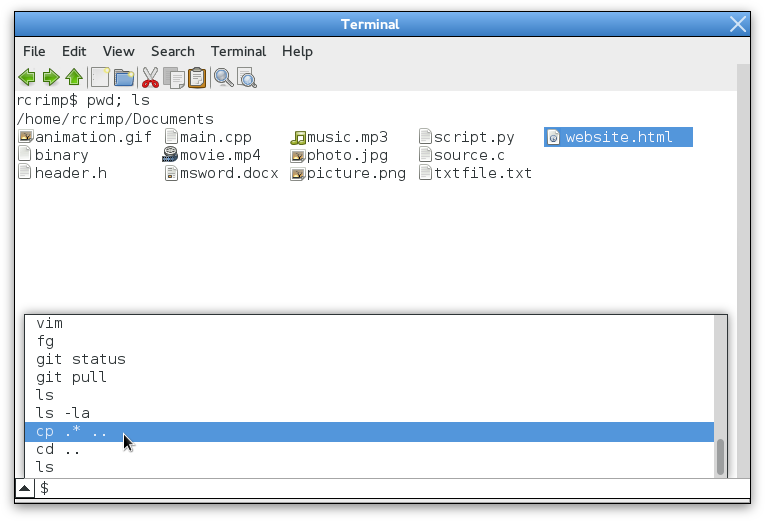
\includegraphics[width=12cm]{history.png}

Fig 2: interactive history\end{center}

\subsection*{Interactive viewing of the command history}
clicking the small arrow to the left of the prompt, will open a drop down menu (upwards), showing the last commands executed in ascending/descending? order (i.e last on bottom). The standard bash style keyboard shortcuts to access your history will also exist for the
more advanced user. (up, down, "", str" etc...)

\subsection*{Directory Bookmarks}
We will allow users to set temporary (and permanent) directory boomarks with a quick command.
\\*executin ``\#work'' will set a boomark in the current directory called "work", and successive execution of the command ``\#work'' will change the users directory back to the first directory in which it was called.
\\\\*i.e. quick navigation between commonly accessed directories when working on a project.

\subsection*{More Advanced Features}

The various forms of ``Tab completion''
tab completion will index: (--decide on an order of precedence--)
 \$PATH
 Path-name completion in the working directory.
 File-name completion in the working directory.
 Path-name completion of all the parent directories of the working directory.
 Variable-name completion
 Man-page completion
 Command history
wild card \*
Tab-Tab lists all possibilities once for each completion, subsequent tabbing will cycle the
prompt through the possibilities.
inline prediction, like googles live search

same line Tab completion i.e like zsh
Utilizes regular expressions
Tab Tab, to list all possible completions

\pagebreak
\section{Script Syntax}

patagraph of words explaining why we chose this langauge
lexically easier to parse?or some shit like that

We will use end statements and colons to delimit program blocks.

\begin{multicols}{2}

\subsubsection*{Keywords}
\begin{tabular}{| l | l | l | l | } \hline
and & break & class & else \\ \hline
end & fail & false & for \\ \hline
function & global & if & in \\ \hline
not & or & print & return \\ \hline
true & try & unicorn & while \\ \hline
\end{tabular}

\subsubsection*{Arithmetic operators}
\begin{tabular}{| l | l | } \hline
+ & Addition \\ \hline
- & Subtraction \\ \hline
a & Multiplication \\ \hline
\textbackslash & Division \\ \hline
\% & Modulus \\ \hline
\textasciicircum  & Exponent \\ \hline
\end{tabular}

\subsubsection*{Assignment operators}
\begin{tabular}{| l | l | } \hline
= & Simple assignment  \\ \hline
+= & Add and assignment  \\ \hline
-= & Subtract and assignment  \\ \hline
\end{tabular}

\subsubsection*{Comparison Operators}
\begin{tabular}{| l | l | } \hline
== & Equal \\ \hline
!= & Not equal \\ \hline
\textgreater & Left larger \\ \hline
\textless & Right Larger \\ \hline
\textgreater= & Left larger than or equal to \\ \hline
\textless= & Right larger than or equal to \\ \hline
\end{tabular}

\end{multicols}

\subsection*{Code Examples}
\begin{multicols}{2}
\subsubsection*{foo function in C}
\begin{lstlisting}
void foo(int x) {
   if (x == 0) {
      bar();
      baz();
   } else {
      quz(x);
      foo(x - 1);
   }
}
\end{lstlisting}
\subsubsection*{foo function in unicorn}
\begin{lstlisting}
function foo(x):
   if x == 0:
      bar()
      baz()
   else:
      qux(x)
      foo(x - 1)
   end
end
\end{lstlisting}
\end{multicols}

\pagebreak
\section{Risk Analysis}

We wanted to implement a proactive approach to dealing with risks as opposed to a reactive approach.

Our objective is to be able to avoid risk whenever possible, and to solve problems before they manifested themselves. This preparation would hopefully mean that we could respond to problems that did occur in a controlled and effective manner. We understand that risks evolve throughout the course of the project and so we will be constantly monitoring identified risks throughout the course of the year via a risk map to ensure that we are still keeping them at bay. 

\section{Project Schedule}

Dependencies between activities - allocation of people to tasks, time until milestones

Monitoring the project and ourselves is an important way for us to anticipate future
problems and gives us a chance to avoid them.
Sticking to the Gant Chart, Pert Chart - make sure on schedule
reporting - GIT hub - so every time we make a build we push it.

((How it will be monitored and when will reports be delivered))
\end{document}
